\subsection[Error Comparison]{$|u - u_h|_{1, \Omega}$ Error Comparison}

Let's now compare the error $|u - u_h|_{1, \Omega}$ between a sequence of uniformly refined meshes and the adaptive method we just defined.

Since there is no mesh size concept for the adaptive refined meshes\footnote{The adaptively refined mesh fails to meet the definition of a quasi-uniform mesh.}, we will compare the errors against the number of elements.

\begin{figure}[!ht]
	\centering
	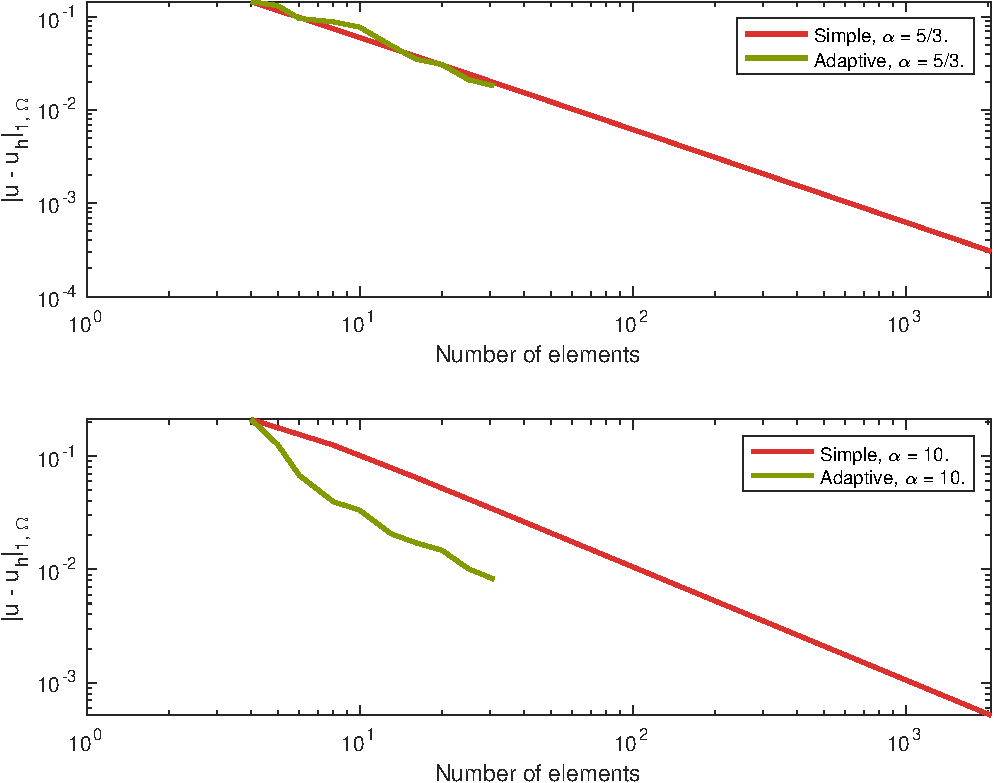
\includegraphics[width=15cm]{comparison.pdf}
	\caption{Comparison between errors against number of elements.}
\end{figure}

As we can see the adaptive method works for both values of $\alpha$, showing great results for $\alpha = 10$ and more or less the same behaviour as the standard method for $\alpha = 5/3$.

\newpage
\begin{multicols}{2}
	\lstinputlisting{../results/comparison.txt}
\end{multicols}

\newpage
\subsection{Stiffness Matrix Conditioning Comparison}

\begin{figure}[!ht]
	\centering
	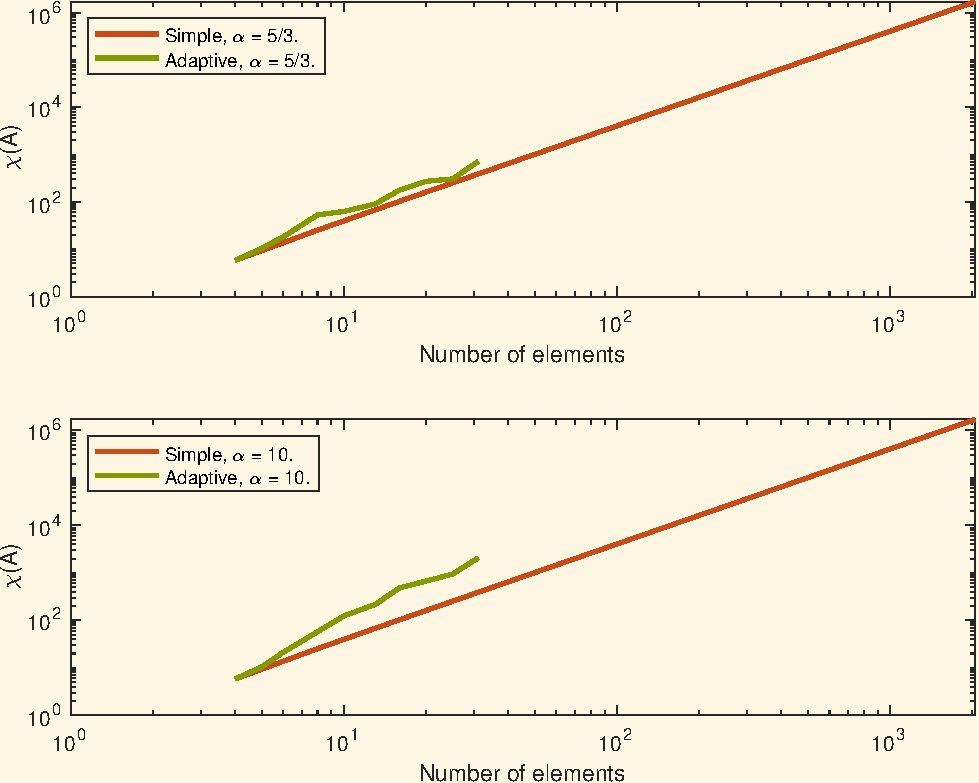
\includegraphics[width=15cm]{comparisonCond.pdf}
	\caption{Comparison between stiffness matrix conditioning against number of elements.}
\end{figure}

\newpage
\begin{multicols}{2}
	\lstinputlisting{../results/comparisonCond.txt}
\end{multicols}